\section{Specifica componenti server}
Package base per le funzionalità del server\begin{center}
	\begin{figure}[H]
		\centering 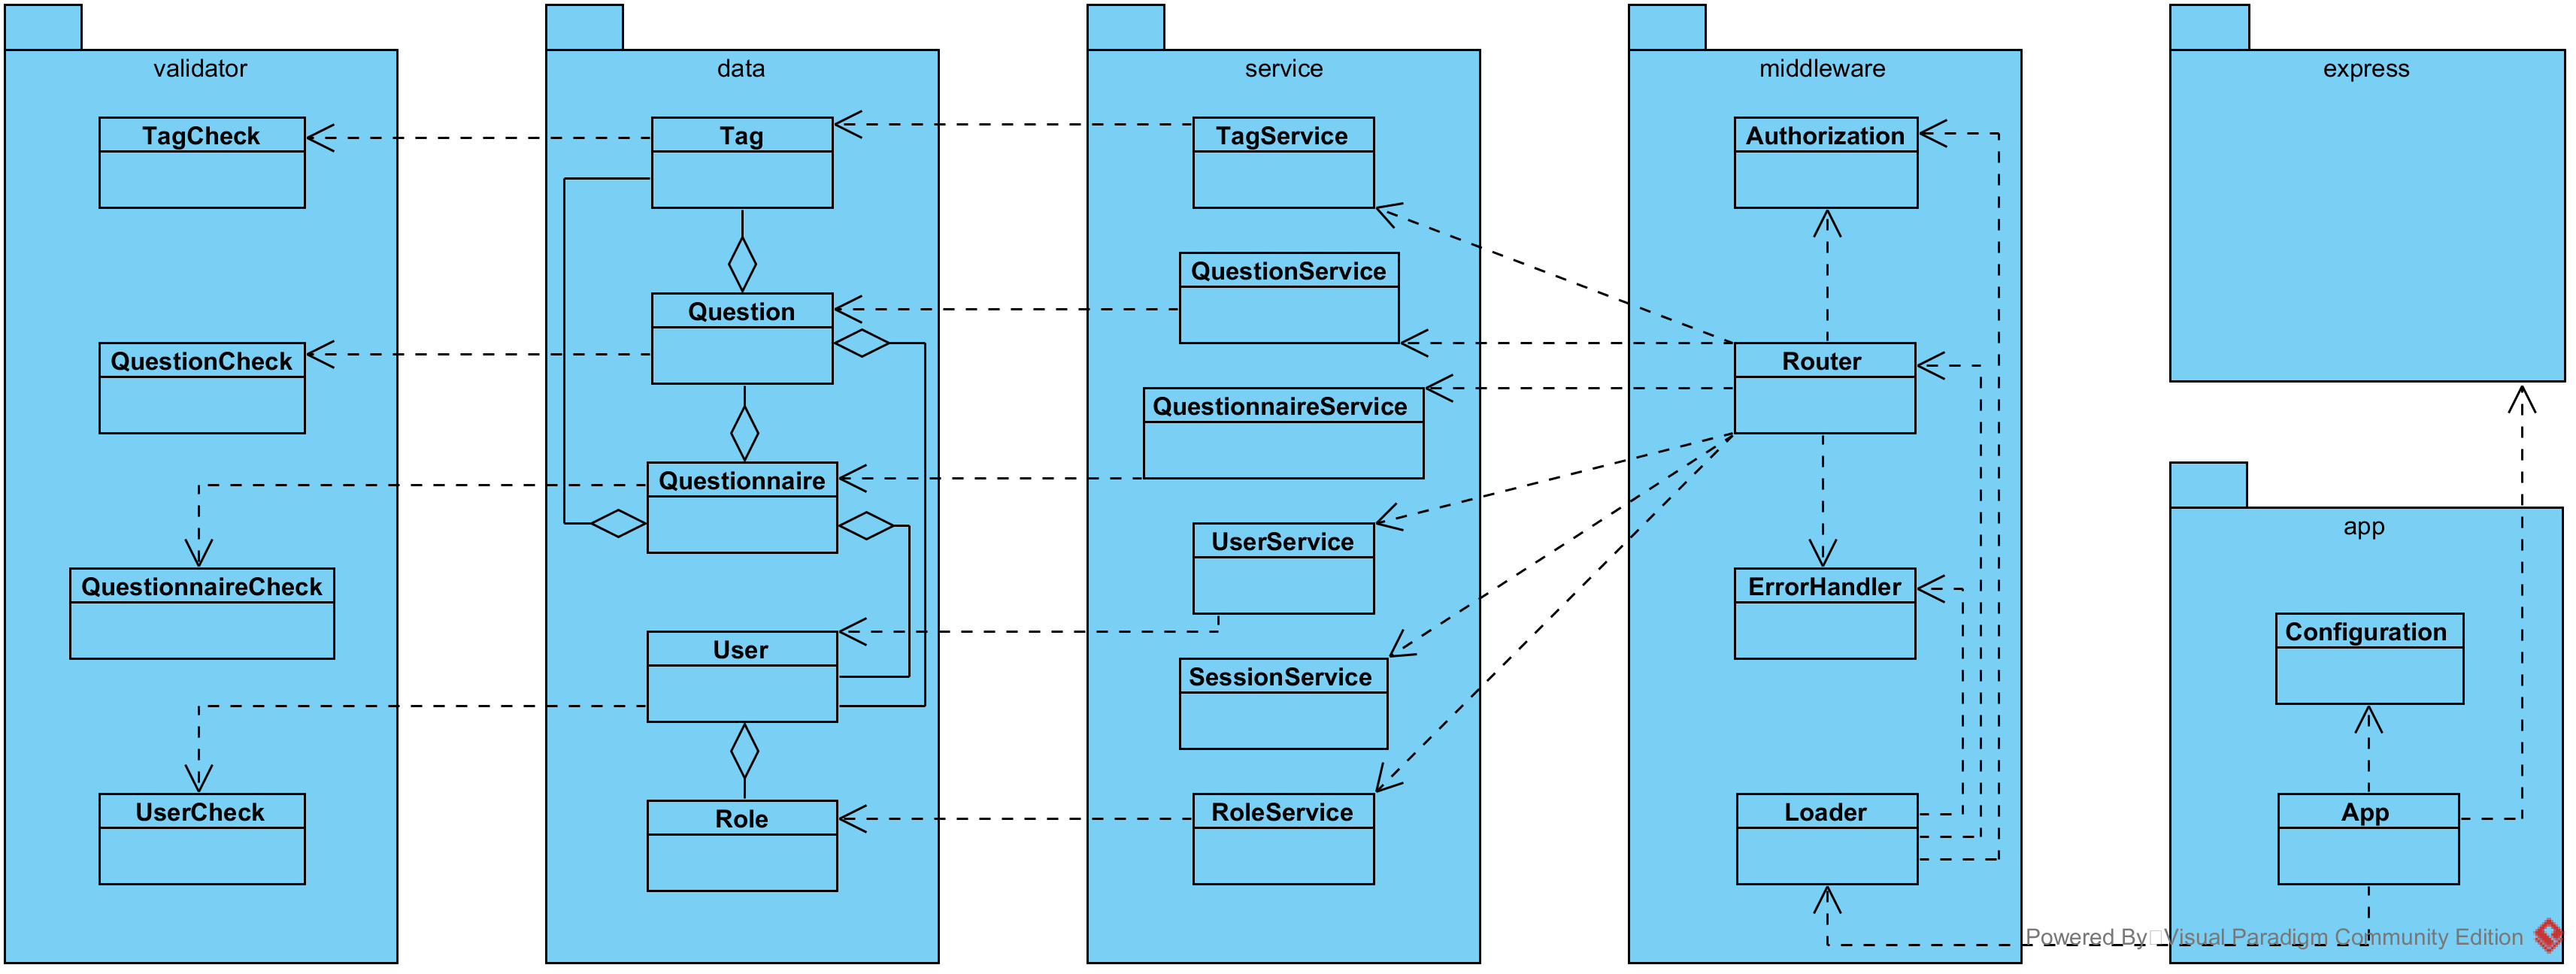
\includegraphics[angle=90, height=20cm]{../img/diagrammiClassi/server.png}
		\caption{Diagramma package - server}
	\end{figure}
\end{center}\subsection{server::app}
Package che ha il compito di fornire i parametri di configurazione e avviare il web server di Quizzipedia\begin{center}
	\begin{figure}[H]
		\centering 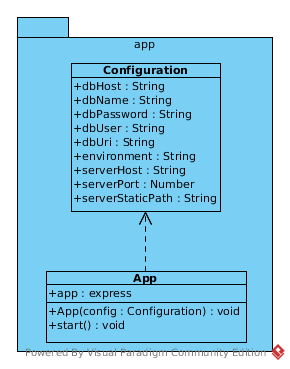
\includegraphics[scale=4, max width=\textwidth, max height=\myheight]{../img/diagrammiClassi/server/app.png}
		\caption{Diagramma package - server::app}
	\end{figure}
\end{center}\hypertarget{server::app::App}{}
\subsubsection[App]{server::app::App}
\begin{figure}[H]
	\centering
	\begin{tikzpicture}
	\umlclass{server::app::App} {--app : Express\\--config : Configuration}{+App(config : Configuration)\\+start() : void\\+config() : Express\\+getApp() : Express\\+setApp(app : Express) : void}
	\end{tikzpicture}
	\caption{Diagramma classe - server::app::App}
\end{figure}\begin{description}
\item[Descrizione] \hfill \\
Classe che si occupa di avviare il server e di invocare i middleware
\item[Utilizzo] \hfill \\
Viene utilizzata per avviare il server dell'applicazione
\item[Relazioni con altre classi] \hfill \\
\vspace{-7mm}
\begin{description}
	\item[\hyperlink{server::app::Configuration}{server::app::Configuration}] \hfill \\
	Relazione uscente, campo dati che rappresenta un riferimento a Configuration
\end{description}

\item[Attributi] \hfill \\
\vspace{-7mm}
\begin{itemize}
	\item app : Express $\rightarrow$ campo dati che rappresenta l'applicazione Express
	\item config : Configuration $\rightarrow$ campo dati che rappresenta un riferimento a Configuration
\end{itemize}

\item[Metodi] \hfill \\
\vspace{-7mm}
\begin{itemize}
	\item App(config : Configuration) $\rightarrow$ costruttore della classe\begin{itemize}
		\item config $\rightarrow$ configurazione per l'inizializzazione dell'applicazione
	\end{itemize}
	
	\item start() : void $\rightarrow$ metodo che avvia il server. Non ritorna il controllo fino a che il server è in funzione
	\item config() : Express $\rightarrow$ metodo che configura i parametri del server sulla base dell'oggetto di configurazione
	\item getApp() : Express $\rightarrow$ metodo che restituisce il valore del campo dati app
	\item setApp(app : Express) : void $\rightarrow$ metodo che cambia il valore del campo dati app\begin{itemize}
		\item app $\rightarrow$ campo dati che rappresenta l'applicazione Express
	\end{itemize}
	
\end{itemize}

\end{description}

\vspace{0.5cm}
\hypertarget{server::app::Configuration}{}
\subsubsection[Configuration]{server::app::Configuration}
\begin{figure}[H]
	\centering
	\begin{tikzpicture}
	\umlclass{server::app::Configuration} {--environment : String\\--serverHost : String\\--serverPort : Number\\--serverStaticPath : String\\--dbHost : String\\--dbName : String\\--dbUser : String\\--dbPassword : String\\--dbUri : String\\--dbPort : number}{+getEnvironment() : String\\+getServerHost() : String\\+getServerPort() : Number\\+getServerStaticPath() : String\\+getDbHost() : String\\+getDbName() : String\\+getDbUser() : String\\+getDbPassword() : String\\+getDbUri() : String\\+getDbPort() : number\\+setEnvironment(environment : String) : void\\+setServerHost(serverHost : String) : void\\+setServerPort(serverPort : Number) : void\\+setServerStaticPath(serverStaticPath : String) : void\\+setDbHost(dbHost : String) : void\\+setDbName(dbName : String) : void\\+setDbUser(dbUser : String) : void\\+setDbPassword(dbPassword : String) : void\\+setDbUri(dbUri : String) : void\\+setDbPort(dbPort : number) : void}
	\end{tikzpicture}
	\caption{Diagramma classe - server::app::Configuration}
\end{figure}\begin{description}
\item[Descrizione] \hfill \\
Classe che contiene tutti i parametri di configurazione necessari al server e all'applicazione Quizzipedia per funzionare
\item[Utilizzo] \hfill \\
Viene utilizzata per definire le configurazioni dell'applicazione, passando un oggetto di questa classe al costruttore della classe App
\item[Relazioni con altre classi] \hfill \\
\vspace{-7mm}
\begin{description}
	\item[\hyperlink{server::app::App}{server::app::App}] \hfill \\
	Relazione entrante, campo dati che rappresenta un riferimento a Configuration
\end{description}

\item[Attributi] \hfill \\
\vspace{-7mm}
\begin{itemize}
	\item environment : String $\rightarrow$ variabile d'ambiente che informa se l'applicazione deve essere eseguita in modalità development o production
	\item serverHost : String $\rightarrow$ campo dati che identifica l'Indirizzo IP dell'host
	\item serverPort : Number $\rightarrow$ campo dati che identifica la porta su cui il server deve mettersi in ascolto
	\item serverStaticPath : String $\rightarrow$ campo dati che identifica il percorso della cartella che il server utilizza per fornire file statici
	\item dbHost : String $\rightarrow$ campo dati che identifica l'host del database
	\item dbName : String $\rightarrow$ campo dati che identifica il nome del database dell'applicazione
	\item dbUser : String $\rightarrow$ campo dati che identifica l'Username per connettersi al database
	\item dbPassword : String $\rightarrow$ campo dati che identifica la password per connettersi al database
	\item dbUri : String $\rightarrow$ campo dati che identifica l'Uri di connessione al database
	\item dbPort : number $\rightarrow$ campo dati che identifica la porta su cui il server di mongodb deve mettersi in ascolto
\end{itemize}

\item[Metodi] \hfill \\
\vspace{-7mm}
\begin{itemize}
	\item getEnvironment() : String $\rightarrow$ metodo che restituisce il valore del campo dati environment
	\item getServerHost() : String $\rightarrow$ metodo che restituisce il valore del campo dati serverHost
	\item getServerPort() : Number $\rightarrow$ metodo che restituisce il valore del campo dati serverPort
	\item getServerStaticPath() : String $\rightarrow$ metodo che restituisce il valore del campo dati serverStaticPath
	\item getDbHost() : String $\rightarrow$ metodo che restituisce il valore del campo dati dbHost
	\item getDbName() : String $\rightarrow$ metodo che restituisce il valore del campo dati dbName
	\item getDbUser() : String $\rightarrow$ metodo che restituisce il valore del campo dati dbUser
	\item getDbPassword() : String $\rightarrow$ metodo che restituisce il valore del campo dati dbPassword
	\item getDbUri() : String $\rightarrow$ metodo che restituisce il valore del campo dati dbUri
	\item getDbPort() : number $\rightarrow$ metodo che restituisce il valore del campo dati dbPort
	\item setEnvironment(environment : String) : void $\rightarrow$ metodo che cambia il valore del campo dati environment\begin{itemize}
		\item environment $\rightarrow$ variabile d'ambiente che informa se l'applicazione deve essere eseguita in modalità development o production
	\end{itemize}
	
	\item setServerHost(serverHost : String) : void $\rightarrow$ metodo che cambia il valore del campo dati serverHost\begin{itemize}
		\item serverHost $\rightarrow$ campo dati che identifica l'Indirizzo IP dell'host
	\end{itemize}
	
	\item setServerPort(serverPort : Number) : void $\rightarrow$ metodo che cambia il valore del campo dati serverPort\begin{itemize}
		\item serverPort $\rightarrow$ campo dati che identifica la porta su cui il server deve mettersi in ascolto
	\end{itemize}
	
	\item setServerStaticPath(serverStaticPath : String) : void $\rightarrow$ metodo che cambia il valore del campo dati serverStaticPath\begin{itemize}
		\item serverStaticPath $\rightarrow$ campo dati che identifica il percorso della cartella che il server utilizza per fornire file statici
	\end{itemize}
	
	\item setDbHost(dbHost : String) : void $\rightarrow$ metodo che cambia il valore del campo dati dbHost\begin{itemize}
		\item dbHost $\rightarrow$ campo dati che identifica l'host del database
	\end{itemize}
	
	\item setDbName(dbName : String) : void $\rightarrow$ metodo che cambia il valore del campo dati dbName\begin{itemize}
		\item dbName $\rightarrow$ campo dati che identifica il nome del database dell'applicazione
	\end{itemize}
	
	\item setDbUser(dbUser : String) : void $\rightarrow$ metodo che cambia il valore del campo dati dbUser\begin{itemize}
		\item dbUser $\rightarrow$ campo dati che identifica l'Username per connettersi al database
	\end{itemize}
	
	\item setDbPassword(dbPassword : String) : void $\rightarrow$ metodo che cambia il valore del campo dati dbPassword\begin{itemize}
		\item dbPassword $\rightarrow$ campo dati che identifica la password per connettersi al database
	\end{itemize}
	
	\item setDbUri(dbUri : String) : void $\rightarrow$ metodo che cambia il valore del campo dati dbUri\begin{itemize}
		\item dbUri $\rightarrow$ campo dati che identifica l'Uri di connessione al database
	\end{itemize}
	
	\item setDbPort(dbPort : number) : void $\rightarrow$ metodo che cambia il valore del campo dati dbPort\begin{itemize}
		\item dbPort $\rightarrow$ campo dati che identifica la porta su cui il server di mongodb deve mettersi in ascolto
	\end{itemize}
	
\end{itemize}

\end{description}

\vspace{0.5cm}
\subsection{server::express}
Express è un framework minimale, basato sul design pattern architetturale MVC per creare applicazioni web con Node.js. Express offre funzionalità che semplificano e aumentano le potenzialità di Node.js, fornendo una migliore implementazione del sistema di routing, incrementando
le funzioni di richiesta e risposta estendendole per una maggior flessibilità, integrando nuovi middleware, ed agevolando la realizzazione delle viste.
Express non limita l’utente nella scelta del linguaggio di templating, lo aiuta a gestire le route, le request e le view\begin{center}
	\begin{figure}[H]
		\centering 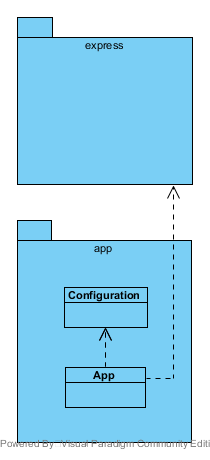
\includegraphics[scale=4, max width=\textwidth, max height=\myheight]{../img/diagrammiClassi/server/expressApp.png}
		\caption{Diagramma package - server::express}
	\end{figure}
\end{center}\subsection{server::middleware}
Package che si occupa di ricevere richieste, richiamare il servizio adatto e restituire le risposte\begin{center}
	\begin{figure}[H]
		\centering 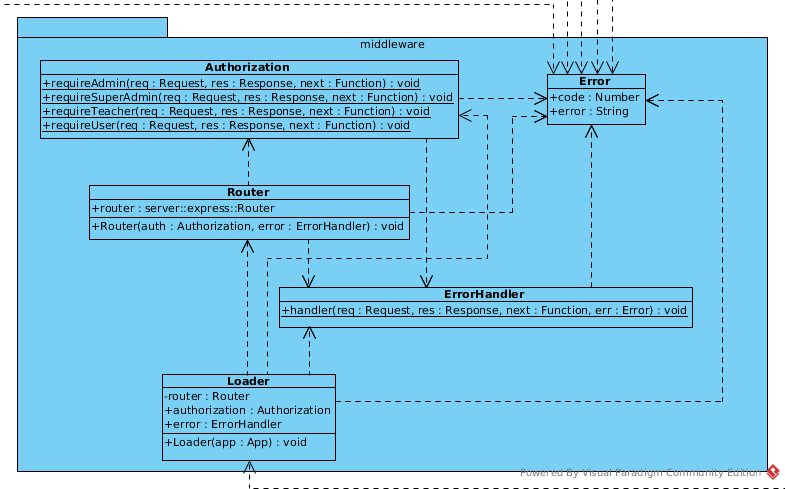
\includegraphics[scale=4, max width=\textwidth, max height=\myheight]{../img/diagrammiClassi/server/middleware.png}
		\caption{Diagramma package - server::middleware}
	\end{figure}
\end{center}\hypertarget{server::middleware::Router}{}
\subsubsection[Router]{server::middleware::Router}
\begin{figure}[H]
	\centering
	\begin{tikzpicture}
	\umlclass{server::middleware::Router} {--router : express.Router\\--sessionService : SessionService\\--userService : UserService\\--questionService : QuestionService\\--questionnaireService : QuestionnaireService\\--tagService : TagService\\--roleService : RoleService\\--answerService : AnswerService}{+Router(auth : Authorization, error : ErrorHandler)}
	\end{tikzpicture}
	\caption{Diagramma classe - server::middleware::Router}
\end{figure}\begin{description}
\item[Descrizione] \hfill \\
Classe che si occupa di instradare le richieste verso le relative richieste
\item[Utilizzo] \hfill \\
Si occupa di smistare la richiesta in base all’URI ricevuto e ad invocare l’opportuno servizio
\item[Relazioni con altre classi] \hfill \\
\vspace{-7mm}
\begin{description}
	\item[\hyperlink{server::service::SessionService}{server::service::SessionService}] \hfill \\
	Relazione uscente, campo dati che rappresenta un oggetto SessionService
	\item[\hyperlink{server::service::UserService}{server::service::UserService}] \hfill \\
	Relazione uscente, campo dati che rappresenta un oggetto UserService
	\item[\hyperlink{server::service::QuestionService}{server::service::QuestionService}] \hfill \\
	Relazione uscente, campo dati che rappresenta un oggetto QuestionService
	\item[\hyperlink{server::service::QuestionnaireService}{server::service::QuestionnaireService}] \hfill \\
	Relazione uscente, campo dati che rappresenta un oggetto QuestionnaireService
	\item[\hyperlink{server::service::TagService}{server::service::TagService}] \hfill \\
	Relazione uscente, campo dati che rappresenta un oggetto TagService
	\item[\hyperlink{server::service::RoleService}{server::service::RoleService}] \hfill \\
	Relazione uscente, campo dati che rappresenta un oggetto RoleService
	\item[\hyperlink{server::middleware::Loader}{server::middleware::Loader}] \hfill \\
	Relazione entrante, campo dati che rappresenta un riferimento al Middleware Router per gestire il reindirizzamento delle richieste
	\item[\hyperlink{server::service::AnswerService}{server::service::AnswerService}] \hfill \\
	Relazione uscente, campo dati che rappresenta un oggetto Answer Service
\end{description}

\item[Attributi] \hfill \\
\vspace{-7mm}
\begin{itemize}
	\item router : express.Router $\rightarrow$ campo dati che rappresenta un oggetto Router di Express
	\item sessionService : SessionService $\rightarrow$ campo dati che rappresenta un oggetto SessionService
	\item userService : UserService $\rightarrow$ campo dati che rappresenta un oggetto UserService
	\item questionService : QuestionService $\rightarrow$ campo dati che rappresenta un oggetto QuestionService
	\item questionnaireService : QuestionnaireService $\rightarrow$ campo dati che rappresenta un oggetto QuestionnaireService
	\item tagService : TagService $\rightarrow$ campo dati che rappresenta un oggetto TagService
	\item roleService : RoleService $\rightarrow$ campo dati che rappresenta un oggetto RoleService
	\item answerService : AnswerService $\rightarrow$ campo dati che rappresenta un oggetto Answer Service
\end{itemize}

\item[Metodi] \hfill \\
\vspace{-7mm}
\begin{itemize}
	\item Router(auth : Authorization, error : ErrorHandler) $\rightarrow$ costruttore della classe\begin{itemize}
		\item auth $\rightarrow$ istanza dell'oggetto Authorization
		\item error $\rightarrow$ istanza del gestore degli errori
	\end{itemize}
	
\end{itemize}

\end{description}

\vspace{0.5cm}
\hypertarget{server::middleware::Authorization}{}
\subsubsection[Authorization]{server::middleware::Authorization}
\begin{figure}[H]
	\centering
	\begin{tikzpicture}
	\umlclass{server::middleware::Authorization} {}{+requireRole(name : String) : Function\\+Authorization()}
	\end{tikzpicture}
	\caption{Diagramma classe - server::middleware::Authorization}
\end{figure}\begin{description}
\item[Descrizione] \hfill \\
Classe che si occupa dell’autorizzazione delle richieste
\item[Utilizzo] \hfill \\
Viene utilizzata per verificare i permessi dell'utente per ogni richiesta
\item[Relazioni con altre classi] \hfill \\
\vspace{-7mm}
\begin{description}
	\item[\hyperlink{server::middleware::Loader}{server::middleware::Loader}] \hfill \\
	Relazione entrante, campo dati che rappresenta un riferimento al Middleware Authorization, utilizzato per l'autorizzazione delle richieste
\end{description}

\item[Metodi] \hfill \\
\vspace{-7mm}
\begin{itemize}
	\item requireRole(name : String) : Function $\rightarrow$ metodo che verifica che l’utente autenticato sia almeno di ruolo specificato, richiamando il successivo middleware in caso affermativo, rispondendo con un errore altrimenti\begin{itemize}
		\item name $\rightarrow$ il nome del ruolo minimo richiesto
	\end{itemize}
	
	\item Authorization() $\rightarrow$ costruttore della classe
\end{itemize}

\end{description}

\vspace{0.5cm}
\hypertarget{server::middleware::Loader}{}
\subsubsection[Loader]{server::middleware::Loader}
\begin{figure}[H]
	\centering
	\begin{tikzpicture}
	\umlclass{server::middleware::Loader} {--authorization : Authorization\\--error : ErrorHandler\\--router : Router}{+Loader(app : App)}
	\end{tikzpicture}
	\caption{Diagramma classe - server::middleware::Loader}
\end{figure}\begin{description}
\item[Descrizione] \hfill \\
Classe utilizzata per istanziare tutti i middleware dell'applicazione
\item[Utilizzo] \hfill \\
Viene utilizzato per istanziare in modo nascosto all’applicazione tutti i middleware presenti nel componente server::middleware
\item[Relazioni con altre classi] \hfill \\
\vspace{-7mm}
\begin{description}
	\item[\hyperlink{server::middleware::Authorization}{server::middleware::Authorization}] \hfill \\
	Relazione uscente, campo dati che rappresenta un riferimento al Middleware Authorization, utilizzato per l'autorizzazione delle richieste. Il Loader si occupa di instanziare questa classe
	\item[\hyperlink{server::middleware::Router}{server::middleware::Router}] \hfill \\
	Relazione uscente, campo dati che rappresenta un riferimento al Middleware Router per gestire il reindirizzamento delle richieste. Il Loader si occupa di instanziare questa classe
	\item[\hyperlink{server::middleware::ErrorHandler}{server::middleware::ErrorHandler}] \hfill \\
	Relazione uscente, campo dati che rappresenta un riferimento al Middleware ErrorHandler, che si occupa di inoltrare le risposte d'errore al client. Il Loader si occupa di instanziare questa classe
\end{description}

\item[Attributi] \hfill \\
\vspace{-7mm}
\begin{itemize}
	\item authorization : Authorization $\rightarrow$ campo dati che rappresenta un riferimento al Middleware Authorization, utilizzato per l'autorizzazione delle richieste
	\item error : ErrorHandler $\rightarrow$ campo dati che rappresenta un riferimento al Middleware ErrorHandler, che si occupa di inoltrare le risposte d'errore al client
	\item router : Router $\rightarrow$ campo dati che rappresenta un riferimento al Middleware Router per gestire il reindirizzamento delle richieste
\end{itemize}

\item[Metodi] \hfill \\
\vspace{-7mm}
\begin{itemize}
	\item Loader(app : App) $\rightarrow$ costruttore della classe\begin{itemize}
		\item app $\rightarrow$ applicazione su cui configurare i middleware
	\end{itemize}
	
\end{itemize}

\end{description}

\vspace{0.5cm}
\hypertarget{server::middleware::ErrorHandler}{}
\subsubsection[ErrorHandler]{server::middleware::ErrorHandler}
\begin{figure}[H]
	\centering
	\begin{tikzpicture}
	\umlclass{server::middleware::ErrorHandler} {}{+handler(req : Request, res : Response, next : Function, err : Error) : void\\+ErrorHandler()}
	\end{tikzpicture}
	\caption{Diagramma classe - server::middleware::ErrorHandler}
\end{figure}\begin{description}
\item[Descrizione] \hfill \\
Classe che gestisce gli errori generati nei controllers restituendo al client la risposta contenente il codice dell'errore verificatosi
\item[Utilizzo] \hfill \\
Questo middleware viene utilizzato per ultimo nella catena di gestione delle richieste di Express, in modo da gestire tutti gli errori generati precedentemente
\item[Relazioni con altre classi] \hfill \\
\vspace{-7mm}
\begin{description}
	\item[\hyperlink{server::middleware::Loader}{server::middleware::Loader}] \hfill \\
	Relazione entrante, campo dati che rappresenta un riferimento al Middleware ErrorHandler, che si occupa di inoltrare le risposte d'errore al client
\end{description}

\item[Metodi] \hfill \\
\vspace{-7mm}
\begin{itemize}
	\item handler(req : Request, res : Response, next : Function, err : Error) : void $\rightarrow$ metodo che gestisce l'errore generato dalla richiesta e da la relativa risposta con il codice dell'errore al client\begin{itemize}
		\item req $\rightarrow$ questo oggetto rappresenta la richiesta arrivata al server che il metodo deve gestire	
		\item res $\rightarrow$ questo oggetto rappresenta la risposta che il server dovrà inviare al termine dell'elaborazione	
		\item next $\rightarrow$ questo parametro rappresenta la callback che il metodo dovrà chiamare al termine dell’elaborazione	
		\item err $\rightarrow$ questo parametro rappresenta l'oggetto  dell'errore
	\end{itemize}
	
	\item ErrorHandler() $\rightarrow$ costruttore della classe
\end{itemize}

\end{description}

\vspace{0.5cm}
\subsection{server::data}
Package contenente le componenti che gestiscono i dati utilizzati dall'applicazione e l'interfacciamento con il database\begin{center}
	\begin{figure}[H]
		\centering 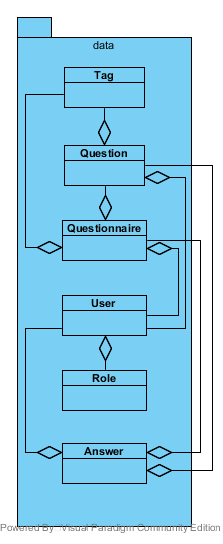
\includegraphics[scale=4, max width=\textwidth, max height=\myheight]{../img/diagrammiClassi/server/data.png}
		\caption{Diagramma package - server::data}
	\end{figure}
\end{center}\hypertarget{server::data::Tag}{}
\subsubsection[Tag]{server::data::Tag}
\begin{figure}[H]
	\centering
	\begin{tikzpicture}
	\umlclass{server::data::Tag} {--name : String\\--description : String}{+getName() : String\\+getDescription() : String\\+setName(name : String) : void\\+setDescription(description : String) : void}
	\end{tikzpicture}
	\caption{Diagramma classe - server::data::Tag}
\end{figure}\begin{description}
\item[Descrizione] \hfill \\
Classe che rappresenta una String contenente l'argomento da assegnare alle domande o ai questionari
\item[Relazioni con altre classi] \hfill \\
\vspace{-7mm}
\begin{description}
	\item[\hyperlink{server::data::Question}{server::data::Question}] \hfill \\
	Relazione entrante, campo dati che rappresenta l'insieme di riferimenti agli argomenti associati alla domanda
	\item[\hyperlink{server::data::Questionnaire}{server::data::Questionnaire}] \hfill \\
	Relazione entrante, campo dati che rappresenta l'insieme di riferimenti agli argomenti associati al questionario
\end{description}

\item[Attributi] \hfill \\
\vspace{-7mm}
\begin{itemize}
	\item name : String $\rightarrow$ campo dati contenente le parole dell'argomento separate da '-'
	\item description : String $\rightarrow$ campo dati che rappresenta una breve descrizione dell'attributo
\end{itemize}

\item[Metodi] \hfill \\
\vspace{-7mm}
\begin{itemize}
	\item getName() : String $\rightarrow$ restituisce il nome identificativo dell'argomento
	\item getDescription() : String $\rightarrow$ restituisce la descrizione dell'argomento
	\item setName(name : String) : void $\rightarrow$ modifica il nome identificativo dell'argomento\begin{itemize}
		\item name $\rightarrow$ campo dati contenente le parole dell'argomento separate da '-'
	\end{itemize}
	
	\item setDescription(description : String) : void $\rightarrow$ imposta la descrizione dell'argomento\begin{itemize}
		\item description $\rightarrow$ campo dati che rappresenta una breve descrizione dell'attributo
	\end{itemize}
	
\end{itemize}

\end{description}

\vspace{0.5cm}
\hypertarget{server::data::Questionnaire}{}
\subsubsection[Questionnaire]{server::data::Questionnaire}
\begin{figure}[H]
	\centering
	\begin{tikzpicture}
	\umlclass{server::data::Questionnaire} {--title : String\\--tags : Tag []\\--author : User\\--questions : Question []}{+getTitle() : String\\+getTags() : Tag []\\+getAuthor() : User\\+getQuestions() : Question []\\+setTitle(title : String) : void\\+setTags(tags : Tag []) : void\\+setQuestions(questions : Question []) : void}
	\end{tikzpicture}
	\caption{Diagramma classe - server::data::Questionnaire}
\end{figure}\begin{description}
\item[Descrizione] \hfill \\
Classe che rappresenta un questionario
\item[Relazioni con altre classi] \hfill \\
\vspace{-7mm}
\begin{description}
	\item[\hyperlink{server::data::Question}{server::data::Question}] \hfill \\
	Relazione uscente, campo dati che rappresenta l'insieme di riferimenti alle domande del questionario
	\item[\hyperlink{server::data::Tag}{server::data::Tag}] \hfill \\
	Relazione uscente, campo dati che rappresenta l'insieme di riferimenti agli argomenti associati al questionario
	\item[\hyperlink{server::data::User}{server::data::User}] \hfill \\
	Relazione uscente, campo dati che rappresenta il riferimento all'autore del questionario
	\item[\hyperlink{server::data::Answer}{server::data::Answer}] \hfill \\
	Relazione entrante, campo dati che rappresenta il questionario della domanda a cui la risposta fa riferimento
\end{description}

\item[Attributi] \hfill \\
\vspace{-7mm}
\begin{itemize}
	\item title : String $\rightarrow$ campo dati che rappresenta il titolo del questionario
	\item tags : Tag [] $\rightarrow$ campo dati che rappresenta l'insieme di riferimenti agli argomenti associati al questionario
	\item author : User $\rightarrow$ campo dati che rappresenta il riferimento all'autore del questionario
	\item questions : Question [] $\rightarrow$ campo dati che rappresenta l'insieme di riferimenti alle domande del questionario
\end{itemize}

\item[Metodi] \hfill \\
\vspace{-7mm}
\begin{itemize}
	\item getTitle() : String $\rightarrow$ restituisce il titolo del questionario
	\item getTags() : Tag [] $\rightarrow$ restituisce la lista dei riferimenti agli argomenti del questionario
	\item getAuthor() : User $\rightarrow$ restituisce il riferimento all'autore del questionario
	\item getQuestions() : Question [] $\rightarrow$ restituisce la lista dei riferimenti alle domande del questionario
	\item setTitle(title : String) : void $\rightarrow$ imposta il titolo del questionario\begin{itemize}
		\item title $\rightarrow$ campo dati che rappresenta il titolo del questionario
	\end{itemize}
	
	\item setTags(tags : Tag []) : void $\rightarrow$ imposta la lista dei riferimenti agli argomenti del questionario\begin{itemize}
		\item tags $\rightarrow$ campo dati che rappresenta l'insieme di riferimenti agli argomenti associati al questionario
	\end{itemize}
	
	\item setQuestions(questions : Question []) : void $\rightarrow$ imposta la lista dei riferimenti alle domande del questionario\begin{itemize}
		\item questions $\rightarrow$ campo dati che rappresenta l'insieme di riferimenti alle domande del questionario
	\end{itemize}
	
\end{itemize}

\end{description}

\vspace{0.5cm}
\hypertarget{server::data::Question}{}
\subsubsection[Question]{server::data::Question}
\begin{figure}[H]
	\centering
	\begin{tikzpicture}
	\umlclass{server::data::Question} {--body : String\\--author : User\\--tags : Tag []}{+getBody() : String\\+getAuthor() : User\\+getTags() : Tag []\\+setBody(body : String) : void\\+setTags(tags : Tag []) : void}
	\end{tikzpicture}
	\caption{Diagramma classe - server::data::Question}
\end{figure}\begin{description}
\item[Descrizione] \hfill \\
Classe base comune a tutti i tipi di domanda
\item[Relazioni con altre classi] \hfill \\
\vspace{-7mm}
\begin{description}
	\item[\hyperlink{server::data::Tag}{server::data::Tag}] \hfill \\
	Relazione uscente, campo dati che rappresenta l'insieme di riferimenti agli argomenti associati alla domanda
	\item[\hyperlink{server::data::User}{server::data::User}] \hfill \\
	Relazione uscente, campo dati che rappresenta il riferimento al docente che ha creato la domanda
	\item[\hyperlink{server::data::Questionnaire}{server::data::Questionnaire}] \hfill \\
	Relazione entrante, campo dati che rappresenta l'insieme di riferimenti alle domande del questionario
	\item[\hyperlink{server::data::Answer}{server::data::Answer}] \hfill \\
	Relazione entrante, campo dati che rappresenta la domanda a cui si riferisce la risposta
\end{description}

\item[Attributi] \hfill \\
\vspace{-7mm}
\begin{itemize}
	\item body : String $\rightarrow$ campo dati che rappresenta il QML del corpo della domanda
	\item author : User $\rightarrow$ campo dati che rappresenta il riferimento al docente che ha creato la domanda
	\item tags : Tag [] $\rightarrow$ campo dati che rappresenta l'insieme di riferimenti agli argomenti associati alla domanda
\end{itemize}

\item[Metodi] \hfill \\
\vspace{-7mm}
\begin{itemize}
	\item getBody() : String $\rightarrow$ restituisce il corpo della domanda in formato QML
	\item getAuthor() : User $\rightarrow$ restituisce il riferimento all'autore della domanda
	\item getTags() : Tag [] $\rightarrow$ restituisce la lista dei riferimenti agli argomenti della domanda
	\item setBody(body : String) : void $\rightarrow$ imposta il corto della domanda in formato QML\begin{itemize}
		\item body $\rightarrow$ campo dati che rappresenta il QML del corpo della domanda
	\end{itemize}
	
	\item setTags(tags : Tag []) : void $\rightarrow$ imposta la lista dei riferimenti agli argomenti della domanda\begin{itemize}
		\item tags $\rightarrow$ campo dati che rappresenta l'insieme di riferimenti agli argomenti associati alla domanda
	\end{itemize}
	
\end{itemize}

\end{description}

\vspace{0.5cm}
\hypertarget{server::data::Role}{}
\subsubsection[Role]{server::data::Role}
\begin{figure}[H]
	\centering
	\begin{tikzpicture}
	\umlclass{server::data::Role} {--name : String}{+greaterThan(role : Role) : boolean\\+equalTo(role : Role) : boolean\\+getName() : String}
	\end{tikzpicture}
	\caption{Diagramma classe - server::data::Role}
\end{figure}\begin{description}
\item[Descrizione] \hfill \\
Classe che rappresenta un ruolo all'interno dell'applicazione
\item[Relazioni con altre classi] \hfill \\
\vspace{-7mm}
\begin{description}
	\item[\hyperlink{server::data::User}{server::data::User}] \hfill \\
	Relazione entrante, campo dati che rappresenta il riferimento al Role dell'utente nell'applicazione
\end{description}

\item[Attributi] \hfill \\
\vspace{-7mm}
\begin{itemize}
	\item name : String $\rightarrow$ campo dati che identifica la tipologia di utente
\end{itemize}

\item[Metodi] \hfill \\
\vspace{-7mm}
\begin{itemize}
	\item greaterThan(role : Role) : boolean $\rightarrow$ metodo che controlla se il ruolo è superiore (e non uguale) a quello passato\begin{itemize}
		\item role $\rightarrow$ l'altro ruolo da comparare
	\end{itemize}
	
	\item equalTo(role : Role) : boolean $\rightarrow$ metodo che controlla se il ruolo è uguale a quello passato\begin{itemize}
		\item role $\rightarrow$ l'altro ruolo da comparare
	\end{itemize}
	
	\item getName() : String $\rightarrow$ restituisce il nome identificativo del ruolo
\end{itemize}

\end{description}

\vspace{0.5cm}
\hypertarget{server::data::User}{}
\subsubsection[User]{server::data::User}
\begin{figure}[H]
	\centering
	\begin{tikzpicture}
	\umlclass{server::data::User} {--fullName : String\\--role : Role\\--userName : String\\--password : String\\--isActive : boolean}{+hasPassword(rawPassword : String) : boolean\\+getFullName() : String\\+getRole() : Role\\+getUserName() : String\\+getIsActive() : boolean\\+setFullName(fullName : String) : void\\+setRole(role : Role) : void\\+setUserName(userName : String) : void\\+setPassword(password : String) : void\\+setIsActive(isActive : boolean) : void}
	\end{tikzpicture}
	\caption{Diagramma classe - server::data::User}
\end{figure}\begin{description}
\item[Descrizione] \hfill \\
Classe che rappresenta un utente dell'applicazione
\item[Relazioni con altre classi] \hfill \\
\vspace{-7mm}
\begin{description}
	\item[\hyperlink{server::data::Question}{server::data::Question}] \hfill \\
	Relazione entrante, campo dati che rappresenta il riferimento al docente che ha creato la domanda
	\item[\hyperlink{server::data::Questionnaire}{server::data::Questionnaire}] \hfill \\
	Relazione entrante, campo dati che rappresenta il riferimento all'autore del questionario
	\item[\hyperlink{server::data::Role}{server::data::Role}] \hfill \\
	Relazione uscente, campo dati che rappresenta il riferimento al Role dell'utente nell'applicazione
	\item[\hyperlink{server::data::Answer}{server::data::Answer}] \hfill \\
	Relazione entrante, campo dati che rappresenta l'autore della risposta
\end{description}

\item[Attributi] \hfill \\
\vspace{-7mm}
\begin{itemize}
	\item fullName : String $\rightarrow$ campo dati che rappresenta il nome e cognome dell'utente
	\item role : Role $\rightarrow$ campo dati che rappresenta il riferimento al Role dell'utente nell'applicazione
	\item userName : String $\rightarrow$ campo dati che rappresenta l'Username univoco con la quale, in combinazione con la password, l'utente accede al sistema
	\item password : String $\rightarrow$ campo dati contenente l'hash della password utilizzata per l'accesso
	\item isActive : boolean $\rightarrow$ campo dati che definisce se l'utente è attivo all'interno del sistema o se è stato disattivato
\end{itemize}

\item[Metodi] \hfill \\
\vspace{-7mm}
\begin{itemize}
	\item hasPassword(rawPassword : String) : boolean $\rightarrow$ metodo che controlla se la password dell'utente è uguale a quella passata\begin{itemize}
		\item rawPassword $\rightarrow$ la password in chiaro
	\end{itemize}
	
	\item getFullName() : String $\rightarrow$ restituisce la stringa rappresentante il nome e cognome (ed eventuale secondo nome) dell'utente
	\item getRole() : Role $\rightarrow$ restituisce il riferimento al ruolo dell'utente
	\item getUserName() : String $\rightarrow$ restituisce il nome identificativo dell'utente utilizzato per l'accesso al sistema
	\item getIsActive() : boolean $\rightarrow$ restituisce un booleano che rappresenta lo stato dell'utente: false significa che l'utente non è abilitato (a tutti gli effetti è rimosso dal sistema), altrimenti l'utente è abilitato
	\item setFullName(fullName : String) : void $\rightarrow$ imposta il nome completo (nome, secondo nome, cognome) dell'utente\begin{itemize}
		\item fullName $\rightarrow$ campo dati che rappresenta il nome e cognome dell'utente
	\end{itemize}
	
	\item setRole(role : Role) : void $\rightarrow$ imposta il riferimento al ruolo dell'utente\begin{itemize}
		\item role $\rightarrow$ campo dati che rappresenta il riferimento al Role dell'utente nell'applicazione
	\end{itemize}
	
	\item setUserName(userName : String) : void $\rightarrow$ imposta il nome identificativo dell'utente\begin{itemize}
		\item userName $\rightarrow$ campo dati che rappresenta l'Username univoco con la quale, in combinazione con la password, l'utente accede al sistema
	\end{itemize}
	
	\item setPassword(password : String) : void $\rightarrow$ imposta la password dell'utente\begin{itemize}
		\item password $\rightarrow$ campo dati contenente l'hash della password utilizzata per l'accesso
	\end{itemize}
	
	\item setIsActive(isActive : boolean) : void $\rightarrow$ imposta lo stato di attività dell'utente (true = abilitato, false = disabilitato)\begin{itemize}
		\item isActive $\rightarrow$ campo dati che definisce se l'utente è attivo all'interno del sistema o se è stato disattivato
	\end{itemize}
	
\end{itemize}

\end{description}

\vspace{0.5cm}
\hypertarget{server::data::Answer}{}
\subsubsection[Answer]{server::data::Answer}
\begin{figure}[H]
	\centering
	\begin{tikzpicture}
	\umlclass{server::data::Answer} {--question : Question\\--questionnaire : Questionnaire\\--author : User\\--score : Number}{+getQuestion() : Question\\+getQuestionnaire() : Questionnaire\\+getAuthor() : User\\+getScore() : Number}
	\end{tikzpicture}
	\caption{Diagramma classe - server::data::Answer}
\end{figure}\begin{description}
\item[Descrizione] \hfill \\
Classe che rappresenta una risposta ad una domanda di un questionario all'interno dell'applicazione
\item[Relazioni con altre classi] \hfill \\
\vspace{-7mm}
\begin{description}
	\item[\hyperlink{server::data::User}{server::data::User}] \hfill \\
	Relazione uscente, campo dati che rappresenta l'autore della risposta
	\item[\hyperlink{server::data::Question}{server::data::Question}] \hfill \\
	Relazione uscente, campo dati che rappresenta la domanda a cui si riferisce la risposta
	\item[\hyperlink{server::data::Questionnaire}{server::data::Questionnaire}] \hfill \\
	Relazione uscente, campo dati che rappresenta il questionario della domanda a cui la risposta fa riferimento
\end{description}

\item[Attributi] \hfill \\
\vspace{-7mm}
\begin{itemize}
	\item question : Question $\rightarrow$ campo dati che rappresenta la domanda a cui si riferisce la risposta
	\item questionnaire : Questionnaire $\rightarrow$ campo dati che rappresenta il questionario della domanda a cui la risposta fa riferimento
	\item author : User $\rightarrow$ campo dati che rappresenta l'autore della risposta
	\item score : Number $\rightarrow$ campo dati che rappresenta il punteggio ottenuto per la risposta (valore razionale tra 0.0 e 1.0 compresi)
\end{itemize}

\item[Metodi] \hfill \\
\vspace{-7mm}
\begin{itemize}
	\item getQuestion() : Question $\rightarrow$ restituisce il riferimento alla domanda alla quale la risposta è stata data all'interno del questionario
	\item getQuestionnaire() : Questionnaire $\rightarrow$ ritorna il riferimento al questionario all'interno della quale si trova la domanda a cui questa risposta è stata data
	\item getAuthor() : User $\rightarrow$ restituisce il riferimento all'autore della risposta
	\item getScore() : Number $\rightarrow$ ritorna il punteggio normalizzato ottenuto da questa risposta (valore razionale tra 0.0 e 1.0 compresi)
\end{itemize}

\end{description}

\vspace{0.5cm}
\subsection{server::service}
Package contenente le classi che implementano tutti i servizi offerti dall'applicazione lato server\begin{center}
	\begin{figure}[H]
		\centering 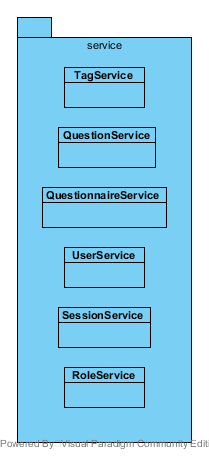
\includegraphics[scale=4, max width=\textwidth, max height=\myheight]{../img/diagrammiClassi/server/service.png}
		\caption{Diagramma package - server::service}
	\end{figure}
\end{center}\hypertarget{server::service::UserService}{}
\subsubsection[UserService]{server::service::UserService}
\begin{figure}[H]
	\centering
	\begin{tikzpicture}
	\umlclass{server::service::UserService} {}{+getByID(req : Request, res : Response, next : Function) : void\\+getMe(req : Request, res : Response, next : Function) : void\\+get(req : Request, res : Response, next : Function) : void\\+new(req : Request, res : Response, next : Function) : void\\+modify(req : Request, res : Response, next : Function) : void\\+delete(req : Request, res : Response, next : Function) : void\\+modifyMe(req : Request, res : Response, next : Function) : void\\+UserService()}
	\end{tikzpicture}
	\caption{Diagramma classe - server::service::UserService}
\end{figure}\begin{description}
\item[Descrizione] \hfill \\
Classe che si occupa della operazioni di inserimento, modifica e rimozione di account utenti, sfruttando la classe server::data::User per accedere ai dati persistenti nel database.
\item[Utilizzo] \hfill \\
Fornisce i dati personali degli utenti a chi ne ha il permesso di accesso ed esegue operazioni di aggiunta, modifica, rimozione e cambio di ruolo per gli utenti del sistema.
\item[Relazioni con altre classi] \hfill \\
\vspace{-7mm}
\begin{description}
	\item[\hyperlink{server::middleware::Router}{server::middleware::Router}] \hfill \\
	Relazione entrante, campo dati che rappresenta un oggetto UserService
\end{description}

\item[Metodi] \hfill \\
\vspace{-7mm}
\begin{itemize}
	\item getByID(req : Request, res : Response, next : Function) : void $\rightarrow$ metodo che ritorna al client un Json contenente l'utente specifico identificato nella richiesta http\begin{itemize}
		\item req $\rightarrow$ questo oggetto rappresenta la richiesta arrivata al server che il metodo deve gestire
		\item res $\rightarrow$ questo oggetto rappresenta la risposta che il server dovrà inviare al termine dell'elaborazione
		\item next $\rightarrow$ questo parametro rappresenta la callback che il metodo dovrà chiamare al termine dell’elaborazione
	\end{itemize}
	
	\item getMe(req : Request, res : Response, next : Function) : void $\rightarrow$ metodo che restituisce al client un Json con i dati relativi all'utente loggato\begin{itemize}
		\item req $\rightarrow$ questo oggetto rappresenta la richiesta arrivata al server che il metodo deve gestire
		\item res $\rightarrow$ questo oggetto rappresenta la risposta che il server dovrà inviare al termine dell'elaborazione
		\item next $\rightarrow$ questo parametro rappresenta la callback che il metodo dovrà chiamare al termine dell’elaborazione
	\end{itemize}
	
	\item get(req : Request, res : Response, next : Function) : void $\rightarrow$ metodo che invia al client la lista degli utenti attraverso un Json\begin{itemize}
		\item req $\rightarrow$ questo oggetto rappresenta la richiesta arrivata al server che il metodo deve gestire
		\item res $\rightarrow$ questo oggetto rappresenta la risposta che il server dovrà inviare al termine dell'elaborazione
		\item next $\rightarrow$ questo parametro rappresenta la callback che il metodo dovrà chiamare al termine dell’elaborazione
	\end{itemize}
	
	\item new(req : Request, res : Response, next : Function) : void $\rightarrow$ metodo che aggiunge un nuovo utente al database\begin{itemize}
		\item req $\rightarrow$ questo oggetto rappresenta la richiesta arrivata al server che il metodo deve gestire
		\item res $\rightarrow$ questo oggetto rappresenta la risposta che il server dovrà inviare al termine dell'elaborazione
		\item next $\rightarrow$ questo parametro rappresenta la callback che il metodo dovrà chiamare al termine dell’elaborazione
	\end{itemize}
	
	\item modify(req : Request, res : Response, next : Function) : void $\rightarrow$ metodo che modifica i dati dell'utente specificato nella richiesta http\begin{itemize}
		\item req $\rightarrow$ questo oggetto rappresenta la richiesta arrivata al server che il metodo deve gestire
		\item res $\rightarrow$ questo oggetto rappresenta la risposta che il server dovrà inviare al termine dell'elaborazione
		\item next $\rightarrow$ questo parametro rappresenta la callback che il metodo dovrà chiamare al termine dell’elaborazione
	\end{itemize}
	
	\item delete(req : Request, res : Response, next : Function) : void $\rightarrow$ metodo che elimina un utente dal database\begin{itemize}
		\item req $\rightarrow$ questo oggetto rappresenta la richiesta arrivata al server che il metodo deve gestire
		\item res $\rightarrow$ questo oggetto rappresenta la risposta che il server dovrà inviare al termine dell'elaborazione
		\item next $\rightarrow$ questo parametro rappresenta la callback che il metodo dovrà chiamare al termine dell’elaborazione
	\end{itemize}
	
	\item modifyMe(req : Request, res : Response, next : Function) : void $\rightarrow$ metodo che modifica i dati dell'utente connesso al sistema se presente\begin{itemize}
		\item req $\rightarrow$ questo oggetto rappresenta la richiesta arrivata al server che il metodo deve gestire
		\item res $\rightarrow$ questo oggetto rappresenta la risposta che il server dovrà inviare al termine dell'elaborazione
		\item next $\rightarrow$ questo parametro rappresenta la callback che il metodo dovrà chiamare al termine dell’elaborazione
	\end{itemize}
	
	\item UserService() $\rightarrow$ costruttore della classe
\end{itemize}

\end{description}

\vspace{0.5cm}
\hypertarget{server::service::QuestionnaireService}{}
\subsubsection[QuestionnaireService]{server::service::QuestionnaireService}
\begin{figure}[H]
	\centering
	\begin{tikzpicture}
	\umlclass{server::service::QuestionnaireService} {}{+getByID(req : Request, res : Response, next : Function) : void\\+get(req : Request, res : Response, next : Function) : void\\+new(req : Request, res : Response, next : Function) : void\\+modify(req : Request, res : Response, next : Function) : void\\+delete(req : Request, res : Response, next : Function) : void\\+QuestionnaireService()}
	\end{tikzpicture}
	\caption{Diagramma classe - server::service::QuestionnaireService}
\end{figure}\begin{description}
\item[Descrizione] \hfill \\
Classe che si occupa di gestire questionari, sfruttando la classe server::data::Questionnaire per accedere ai dati persistenti nel database.
\item[Utilizzo] \hfill \\
Offre metodi per restituire questionari. Permette inoltre ad un docente di effettuare l'inserimento, la modifica, l'eliminazione di questionari
\item[Relazioni con altre classi] \hfill \\
\vspace{-7mm}
\begin{description}
	\item[\hyperlink{server::middleware::Router}{server::middleware::Router}] \hfill \\
	Relazione entrante, campo dati che rappresenta un oggetto QuestionnaireService
\end{description}

\item[Metodi] \hfill \\
\vspace{-7mm}
\begin{itemize}
	\item getByID(req : Request, res : Response, next : Function) : void $\rightarrow$ metodo che ritorna al client un Json contenente il questionario specifico richiesto identificato nella richiesta http\begin{itemize}
		\item req $\rightarrow$ questo oggetto rappresenta la richiesta arrivata al server che il metodo deve gestire
		\item res $\rightarrow$ questo oggetto rappresenta la risposta che il server dovrà inviare al termine dell'elaborazione
		\item next $\rightarrow$ questo parametro rappresenta la callback che il metodo dovrà chiamare al termine dell’elaborazione
	\end{itemize}
	
	\item get(req : Request, res : Response, next : Function) : void $\rightarrow$ metodo che invia al client una lista di questionari attraverso un Json\begin{itemize}
		\item req $\rightarrow$ questo oggetto rappresenta la richiesta arrivata al server che il metodo deve gestire
		\item res $\rightarrow$ questo oggetto rappresenta la risposta che il server dovrà inviare al termine dell'elaborazione
		\item next $\rightarrow$ questo parametro rappresenta la callback che il metodo dovrà chiamare al termine dell’elaborazione
	\end{itemize}
	
	\item new(req : Request, res : Response, next : Function) : void $\rightarrow$ metodo che aggiunge un nuovo questionario al database\begin{itemize}
		\item req $\rightarrow$ questo oggetto rappresenta la richiesta arrivata al server che il metodo deve gestire
		\item res $\rightarrow$ questo oggetto rappresenta la risposta che il server dovrà inviare al termine dell'elaborazione
		\item next $\rightarrow$ questo parametro rappresenta la callback che il metodo dovrà chiamare al termine dell’elaborazione
	\end{itemize}
	
	\item modify(req : Request, res : Response, next : Function) : void $\rightarrow$ metodo che modifica un questionario specificato nella richiesta http\begin{itemize}
		\item req $\rightarrow$ questo oggetto rappresenta la richiesta arrivata al server che il metodo deve gestire
		\item res $\rightarrow$ questo oggetto rappresenta la risposta che il server dovrà inviare al termine dell'elaborazione
		\item next $\rightarrow$ questo parametro rappresenta la callback che il metodo dovrà chiamare al termine dell’elaborazione
	\end{itemize}
	
	\item delete(req : Request, res : Response, next : Function) : void $\rightarrow$ metodo che cancella un questionario specifico dal database\begin{itemize}
		\item req $\rightarrow$ questo oggetto rappresenta la richiesta arrivata al server che il metodo deve gestire
		\item res $\rightarrow$ questo oggetto rappresenta la risposta che il server dovrà inviare al termine dell'elaborazione
		\item next $\rightarrow$ questo parametro rappresenta la callback che il metodo dovrà chiamare al termine dell’elaborazione
	\end{itemize}
	
	\item QuestionnaireService() $\rightarrow$ costruttore della classe
\end{itemize}

\end{description}

\vspace{0.5cm}
\hypertarget{server::service::QuestionService}{}
\subsubsection[QuestionService]{server::service::QuestionService}
\begin{figure}[H]
	\centering
	\begin{tikzpicture}
	\umlclass{server::service::QuestionService} {}{+get(req : Request, res : Response, next : Function) : void\\+getByID(req : Request, res : Response, next : Function) : void\\+new(req : Request, res : Response, next : Function) : void\\+modify(req : Request, res : Response, next : Function) : void\\+delete(req : Request, res : Response, next : Function) : void\\+QuestionService()}
	\end{tikzpicture}
	\caption{Diagramma classe - server::service::QuestionService}
\end{figure}\begin{description}
\item[Descrizione] \hfill \\
Classe che si occupa di gestire domande, sfruttando la classe server::data::Question per accedere ai dati persistenti nel database
\item[Utilizzo] \hfill \\
Offre metodi per restituire le domande. Permette inoltre ad un docente di effettuare l'inserimento, la modifica, l'eliminazione di domande
\item[Relazioni con altre classi] \hfill \\
\vspace{-7mm}
\begin{description}
	\item[\hyperlink{server::middleware::Router}{server::middleware::Router}] \hfill \\
	Relazione entrante, campo dati che rappresenta un oggetto QuestionService
\end{description}

\item[Metodi] \hfill \\
\vspace{-7mm}
\begin{itemize}
	\item get(req : Request, res : Response, next : Function) : void $\rightarrow$ metodo che invia al client una lista di domande attraverso un Json\begin{itemize}
		\item req $\rightarrow$ questo oggetto rappresenta la richiesta arrivata al server che il metodo deve gestire
		\item res $\rightarrow$ questo oggetto rappresenta la risposta che il server dovrà inviare al termine dell'elaborazione
		\item next $\rightarrow$ questo parametro rappresenta la callback che il metodo dovrà chiamare al termine dell’elaborazione
	\end{itemize}
	
	\item getByID(req : Request, res : Response, next : Function) : void $\rightarrow$ metodo che ritorna al client un Json contenente la domanda specifica identificata nella richiesta http\begin{itemize}
		\item req $\rightarrow$ questo oggetto rappresenta la richiesta arrivata al server che il metodo deve gestire
		\item res $\rightarrow$ questo oggetto rappresenta la risposta che il server dovrà inviare al termine dell'elaborazione
		\item next $\rightarrow$ questo parametro rappresenta la callback che il metodo dovrà chiamare al termine dell’elaborazione
	\end{itemize}
	
	\item new(req : Request, res : Response, next : Function) : void $\rightarrow$ metodo che aggiunge una nuova domanda al database\begin{itemize}
		\item req $\rightarrow$ questo oggetto rappresenta la richiesta arrivata al server che il metodo deve gestire
		\item res $\rightarrow$ questo oggetto rappresenta la risposta che il server dovrà inviare al termine dell'elaborazione
		\item next $\rightarrow$ questo parametro rappresenta la callback che il metodo dovrà chiamare al termine dell’elaborazione
	\end{itemize}
	
	\item modify(req : Request, res : Response, next : Function) : void $\rightarrow$ metodo che modifica una domanda specificato nella richiesta http\begin{itemize}
		\item req $\rightarrow$ questo oggetto rappresenta la richiesta arrivata al server che il metodo deve gestire
		\item res $\rightarrow$ questo oggetto rappresenta la risposta che il server dovrà inviare al termine dell'elaborazione
		\item next $\rightarrow$ questo parametro rappresenta la callback che il metodo dovrà chiamare al termine dell’elaborazione
	\end{itemize}
	
	\item delete(req : Request, res : Response, next : Function) : void $\rightarrow$ metodo che elimina una domanda selezionata dal database\begin{itemize}
		\item req $\rightarrow$ questo oggetto rappresenta la richiesta arrivata al server che il metodo deve gestire
		\item res $\rightarrow$ questo oggetto rappresenta la risposta che il server dovrà inviare al termine dell'elaborazione
		\item next $\rightarrow$ questo parametro rappresenta la callback che il metodo dovrà chiamare al termine dell’elaborazione
	\end{itemize}
	
	\item QuestionService() $\rightarrow$ costruttore della classe
\end{itemize}

\end{description}

\vspace{0.5cm}
\hypertarget{server::service::TagService}{}
\subsubsection[TagService]{server::service::TagService}
\begin{figure}[H]
	\centering
	\begin{tikzpicture}
	\umlclass{server::service::TagService} {}{+get(req : Request, res : Response, next : Function) : void\\+getByID(req : Request, res : Response, next : Function) : void\\+new(req : Request, res : Response, next : Function) : void\\+modify(req : Request, res : Response, next : Function) : void\\+delete(req : Request, res : Response, next : Function) : void\\+TagService()}
	\end{tikzpicture}
	\caption{Diagramma classe - server::service::TagService}
\end{figure}\begin{description}
\item[Descrizione] \hfill \\
Classe che si occupa di gestire gli argomenti, sfruttando la classe server::data::Tag per accedere ai dati persistenti nel database
\item[Utilizzo] \hfill \\
Offre metodi per restituire gli argomenti presenti. Permette inoltre ad un docente di effettuare l'inserimento, la modifica, l'eliminazione di argomenti
\item[Relazioni con altre classi] \hfill \\
\vspace{-7mm}
\begin{description}
	\item[\hyperlink{server::middleware::Router}{server::middleware::Router}] \hfill \\
	Relazione entrante, campo dati che rappresenta un oggetto TagService
\end{description}

\item[Metodi] \hfill \\
\vspace{-7mm}
\begin{itemize}
	\item get(req : Request, res : Response, next : Function) : void $\rightarrow$ metodo che invia al client la lista degli argomenti attraverso un Json\begin{itemize}
		\item req $\rightarrow$ questo oggetto rappresenta la richiesta arrivata al server che il metodo deve gestire
		\item res $\rightarrow$ questo oggetto rappresenta la risposta che il server dovrà inviare al termine dell'elaborazione
		\item next $\rightarrow$ questo parametro rappresenta la callback che il metodo dovrà chiamare al termine dell’elaborazione
	\end{itemize}
	
	\item getByID(req : Request, res : Response, next : Function) : void $\rightarrow$ metodo che ritorna al client un Json contenente l'argomento specifico identificato nella richiesta http\begin{itemize}
		\item req $\rightarrow$ questo oggetto rappresenta la richiesta arrivata al server che il metodo deve gestire
		\item res $\rightarrow$ questo oggetto rappresenta la risposta che il server dovrà inviare al termine dell'elaborazione
		\item next $\rightarrow$ questo parametro rappresenta la callback che il metodo dovrà chiamare al termine dell’elaborazione
	\end{itemize}
	
	\item new(req : Request, res : Response, next : Function) : void $\rightarrow$ metodo che aggiunge un nuovo argomento al database\begin{itemize}
		\item req $\rightarrow$ questo oggetto rappresenta la richiesta arrivata al server che il metodo deve gestire
		\item res $\rightarrow$ questo oggetto rappresenta la risposta che il server dovrà inviare al termine dell'elaborazione
		\item next $\rightarrow$ questo parametro rappresenta la callback che il metodo dovrà chiamare al termine dell’elaborazione
	\end{itemize}
	
	\item modify(req : Request, res : Response, next : Function) : void $\rightarrow$ metodo che modifica un argomento specificato nella richiesta http\begin{itemize}
		\item req $\rightarrow$ questo oggetto rappresenta la richiesta arrivata al server che il metodo deve gestire
		\item res $\rightarrow$ questo oggetto rappresenta la risposta che il server dovrà inviare al termine dell'elaborazione
		\item next $\rightarrow$ questo parametro rappresenta la callback che il metodo dovrà chiamare al termine dell’elaborazione
	\end{itemize}
	
	\item delete(req : Request, res : Response, next : Function) : void $\rightarrow$ metodo che elimina un argomento specifico dal database\begin{itemize}
		\item req $\rightarrow$ questo oggetto rappresenta la richiesta arrivata al server che il metodo deve gestire
		\item res $\rightarrow$ questo oggetto rappresenta la risposta che il server dovrà inviare al termine dell'elaborazione
		\item next $\rightarrow$ questo parametro rappresenta la callback che il metodo dovrà chiamare al termine dell’elaborazione
	\end{itemize}
	
	\item TagService() $\rightarrow$ costruttore della classe
\end{itemize}

\end{description}

\vspace{0.5cm}
\hypertarget{server::service::SessionService}{}
\subsubsection[SessionService]{server::service::SessionService}
\begin{figure}[H]
	\centering
	\begin{tikzpicture}
	\umlclass{server::service::SessionService} {}{+new(req : Request, res : Response, next : Function) : void\\+delete(req : Request, res : Response, next : Function) : void\\+SessionService()}
	\end{tikzpicture}
	\caption{Diagramma classe - server::service::SessionService}
\end{figure}\begin{description}
\item[Descrizione] \hfill \\
Classe che si occupa della gestione della sessione dell'utente, sfruttando la classe server::data::User per accedere ai dati persistenti nel database
\item[Utilizzo] \hfill \\
Viene utilizzata per gestire il login e logout dell'utente
\item[Relazioni con altre classi] \hfill \\
\vspace{-7mm}
\begin{description}
	\item[\hyperlink{server::middleware::Router}{server::middleware::Router}] \hfill \\
	Relazione entrante, campo dati che rappresenta un oggetto SessionService
\end{description}

\item[Metodi] \hfill \\
\vspace{-7mm}
\begin{itemize}
	\item new(req : Request, res : Response, next : Function) : void $\rightarrow$ metodo che crea una sessione con una volta che l'utente effettua l'accesso all'applicazione\begin{itemize}
		\item req $\rightarrow$ questo oggetto rappresenta la richiesta arrivata al server che il metodo deve gestire
		\item res $\rightarrow$ questo oggetto rappresenta la risposta che il server dovrà inviare al termine dell'elaborazione
		\item next $\rightarrow$ questo parametro rappresenta la callback che il metodo dovrà chiamare al termine dell’elaborazione
	\end{itemize}
	
	\item delete(req : Request, res : Response, next : Function) : void $\rightarrow$ metodo che elimina la sessione dell'utente dal database\begin{itemize}
		\item req $\rightarrow$ questo oggetto rappresenta la richiesta arrivata al server che il metodo deve gestire
		\item res $\rightarrow$ questo oggetto rappresenta la risposta che il server dovrà inviare al termine dell'elaborazione
		\item next $\rightarrow$ questo parametro rappresenta la callback che il metodo dovrà chiamare al termine dell’elaborazione
	\end{itemize}
	
	\item SessionService() $\rightarrow$ costruttore della classe
\end{itemize}

\end{description}

\vspace{0.5cm}
\hypertarget{server::service::RoleService}{}
\subsubsection[RoleService]{server::service::RoleService}
\begin{figure}[H]
	\centering
	\begin{tikzpicture}
	\umlclass{server::service::RoleService} {}{+get(req : Request, res : Response, next : Function) : void\\+getByID(req : Request, res : Response, next : Function) : void\\+RoleService()}
	\end{tikzpicture}
	\caption{Diagramma classe - server::service::RoleService}
\end{figure}\begin{description}
\item[Descrizione] \hfill \\
Classe che rappresenta il servizio per la lettura dei ruoli utente, sfruttando la classe server::data::Role per accedere ai dati persistenti nel database
\item[Utilizzo] \hfill \\
Viene utilizzata per fornire un punto d'accesso per l'elenco di tutti i ruoli dell'applicazione e la lettura di un singolo ruolo
\item[Relazioni con altre classi] \hfill \\
\vspace{-7mm}
\begin{description}
	\item[\hyperlink{server::middleware::Router}{server::middleware::Router}] \hfill \\
	Relazione entrante, campo dati che rappresenta un oggetto RoleService
\end{description}

\item[Metodi] \hfill \\
\vspace{-7mm}
\begin{itemize}
	\item get(req : Request, res : Response, next : Function) : void $\rightarrow$ metodo che invia al client la lista di tutti i ruoli assumibili dagli utenti dell'applicazione attraverso un Json\begin{itemize}
		\item req $\rightarrow$ questo oggetto rappresenta la richiesta arrivata al server che il metodo deve gestire
		\item res $\rightarrow$ questo oggetto rappresenta la risposta che il server dovrà inviare al termine dell'elaborazione
		\item next $\rightarrow$ questo parametro rappresenta la callback che il metodo dovrà chiamare al termine dell’elaborazione
	\end{itemize}
	
	\item getByID(req : Request, res : Response, next : Function) : void $\rightarrow$ metodo che ritorna al client un Json contenente il ruolo specificato nella richiesta http\begin{itemize}
		\item req $\rightarrow$ questo oggetto rappresenta la richiesta arrivata al server che il metodo deve gestire
		\item res $\rightarrow$ questo oggetto rappresenta la risposta che il server dovrà inviare al termine dell'elaborazione
		\item next $\rightarrow$ questo parametro rappresenta la callback che il metodo dovrà chiamare al termine dell’elaborazione
	\end{itemize}
	
	\item RoleService() $\rightarrow$ costruttore della classe
\end{itemize}

\end{description}

\vspace{0.5cm}
\hypertarget{server::service::AnswerService}{}
\subsubsection[AnswerService]{server::service::AnswerService}
\begin{figure}[H]
	\centering
	\begin{tikzpicture}
	\umlclass{server::service::AnswerService} {}{+get(req : Request, res : Response, next : Function) : void\\+getByID(req : Request, res : Response, next : Function) : void\\+new(req : Request, res : Response, next : Function) : void\\+AnswerService()}
	\end{tikzpicture}
	\caption{Diagramma classe - server::service::AnswerService}
\end{figure}\begin{description}
\item[Descrizione] \hfill \\
Classe che si occupa della operazioni di inserimento e visualizzazione di risposte a domande dei questionari, sfruttando la classe server::data::Answer per accedere ai dati persistenti nel database.
\item[Utilizzo] \hfill \\
Fornisce i punteggi delle risposte date alle domande dei questionari a chi ne ha il permesso di accesso ed esegue operazioni di aggiunta e visualizzazione.
\item[Relazioni con altre classi] \hfill \\
\vspace{-7mm}
\begin{description}
	\item[\hyperlink{server::middleware::Router}{server::middleware::Router}] \hfill \\
	Relazione entrante, campo dati che rappresenta un oggetto Answer Service
\end{description}

\item[Metodi] \hfill \\
\vspace{-7mm}
\begin{itemize}
	\item get(req : Request, res : Response, next : Function) : void $\rightarrow$ metodo che invia al client la lista delle risposte in formato JSON in base alle impostazioni di filtraggio impostate\begin{itemize}
		\item req $\rightarrow$ questo oggetto rappresenta la richiesta arrivata al server che il metodo deve gestire
		\item res $\rightarrow$ questo oggetto rappresenta la risposta che il server dovrà inviare al termine dell'elaborazione
		\item next $\rightarrow$ questo parametro rappresenta la callback che il metodo dovrà chiamare al termine dell’elaborazione
	\end{itemize}
	
	\item getByID(req : Request, res : Response, next : Function) : void $\rightarrow$ metodo che ritorna al client un oggetto JSON contenente i dati della risposta identificata nella richiesta http\begin{itemize}
		\item req $\rightarrow$ questo oggetto rappresenta la richiesta arrivata al server che il metodo deve gestire
		\item res $\rightarrow$ questo oggetto rappresenta la risposta che il server dovrà inviare al termine dell'elaborazione
		\item next $\rightarrow$ questo parametro rappresenta la callback che il metodo dovrà chiamare al termine dell’elaborazione
	\end{itemize}
	
	\item new(req : Request, res : Response, next : Function) : void $\rightarrow$ metodo che aggiunge una nuova risposta nel database\begin{itemize}
		\item req $\rightarrow$ questo oggetto rappresenta la richiesta arrivata al server che il metodo deve gestire
		\item res $\rightarrow$ questo oggetto rappresenta la risposta che il server dovrà inviare al termine dell'elaborazione
		\item next $\rightarrow$ questo parametro rappresenta la callback che il metodo dovrà chiamare al termine dell’elaborazione
	\end{itemize}
	
	\item AnswerService() $\rightarrow$ costruttore della classe
\end{itemize}

\end{description}

\vspace{0.5cm}
\subsection{server::validator}
Package contenente tutte le classi "validator" che hanno il compito di controllare che alcuni campi di alcuni model siano validi; esempi includono la password dell'utente, la lunghezza del nome utente o il QML di una domanda\begin{center}
	\begin{figure}[H]
		\centering 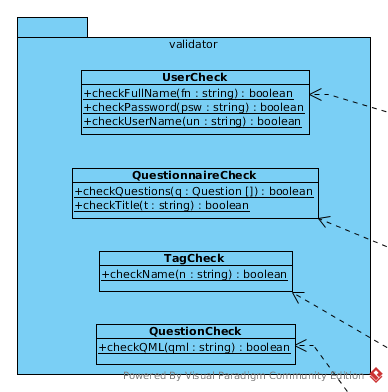
\includegraphics[scale=4, max width=\textwidth, max height=\myheight]{../img/diagrammiClassi/server/validator.png}
		\caption{Diagramma package - server::validator}
	\end{figure}
\end{center}\hypertarget{server::validator::UserCheck}{}
\subsubsection[UserCheck]{server::validator::UserCheck}
\begin{figure}[H]
	\centering
	\begin{tikzpicture}
	\umlclass{server::validator::UserCheck} {}{+checkFullName(fullName : String) : boolean\\+checkPassword(psw : String) : boolean\\+checkUserName(userName : String) : boolean\\+UserCheck()}
	\end{tikzpicture}
	\caption{Diagramma classe - server::validator::UserCheck}
\end{figure}\begin{description}
\item[Descrizione] \hfill \\
Classe contenente tutte le funzioni di controllo della validità dei campi del model User
\item[Utilizzo] \hfill \\
Viene utilizzata dai service per effettuare controlli sul model User
\item[Metodi] \hfill \\
\vspace{-7mm}
\begin{itemize}
	\item checkFullName(fullName : String) : boolean $\rightarrow$ metodo che controlla che il nome completo passato contenga almeno 2 caratteri\begin{itemize}
		\item fullName $\rightarrow$ il nome completo da controllare
	\end{itemize}
	
	\item checkPassword(psw : String) : boolean $\rightarrow$ metodo che controlla che la password passata contenga almeno 6 caratteri\begin{itemize}
		\item psw $\rightarrow$ la password, ovviamente in chiaro (non l'hash), da controllare
	\end{itemize}
	
	\item checkUserName(userName : String) : boolean $\rightarrow$ metodo che controlla che l'username passato contenga almeno 6 caratteri\begin{itemize}
		\item userName $\rightarrow$ l'username da controllare
	\end{itemize}
	
	\item UserCheck() $\rightarrow$ costruttore della classe
\end{itemize}

\end{description}

\vspace{0.5cm}
\hypertarget{server::validator::QuestionnaireCheck}{}
\subsubsection[QuestionnaireCheck]{server::validator::QuestionnaireCheck}
\begin{figure}[H]
	\centering
	\begin{tikzpicture}
	\umlclass{server::validator::QuestionnaireCheck} {}{+checkQuestions(questions : Question []) : boolean\\+checkTitle(title : String) : boolean\\+checkTags(tags : Tag []) : boolean\\+QuestionnaireCheck()}
	\end{tikzpicture}
	\caption{Diagramma classe - server::validator::QuestionnaireCheck}
\end{figure}\begin{description}
\item[Descrizione] \hfill \\
Classe contenente tutte le funzioni di controllo della validità dei campi del model Questionnaire
\item[Utilizzo] \hfill \\
Viene utilizzata dai service per effettuare controlli sul model User
\item[Metodi] \hfill \\
\vspace{-7mm}
\begin{itemize}
	\item checkQuestions(questions : Question []) : boolean $\rightarrow$ metodo che controlla che la lista/array di domande passate non sia vuota e che non contenga domande duplicate\begin{itemize}
		\item questions $\rightarrow$ l'elenco delle domande del questionario
	\end{itemize}
	
	\item checkTitle(title : String) : boolean $\rightarrow$ metodo che controlla che il titolo del questionario non sia vuoto\begin{itemize}
		\item title $\rightarrow$ il titolo del questionario da controllare
	\end{itemize}
	
	\item checkTags(tags : Tag []) : boolean $\rightarrow$ metodo che controlla che la lista/array di argomenti passati non sia vuota\begin{itemize}
		\item tags $\rightarrow$ elenco degli argomenti	
	\end{itemize}
	
	\item QuestionnaireCheck() $\rightarrow$ costruttore della classe
\end{itemize}

\end{description}

\vspace{0.5cm}
\hypertarget{server::validator::TagCheck}{}
\subsubsection[TagCheck]{server::validator::TagCheck}
\begin{figure}[H]
	\centering
	\begin{tikzpicture}
	\umlclass{server::validator::TagCheck} {}{+checkName(name : String) : boolean\\+TagCheck()}
	\end{tikzpicture}
	\caption{Diagramma classe - server::validator::TagCheck}
\end{figure}\begin{description}
\item[Descrizione] \hfill \\
Classe contenente tutte le funzioni di controllo della validità dei campi del model Tag
\item[Utilizzo] \hfill \\
Viene utilizzata dai service per effettuare controlli sul model Tag
\item[Metodi] \hfill \\
\vspace{-7mm}
\begin{itemize}
	\item checkName(name : String) : boolean $\rightarrow$ metodo che controlla che il nome dell'argomento non sia vuoto\begin{itemize}
		\item name $\rightarrow$ il nome dell'argomento da controllare
	\end{itemize}
	
	\item TagCheck() $\rightarrow$ costruttore della classe
\end{itemize}

\end{description}

\vspace{0.5cm}
\hypertarget{server::validator::QuestionCheck}{}
\subsubsection[QuestionCheck]{server::validator::QuestionCheck}
\begin{figure}[H]
	\centering
	\begin{tikzpicture}
	\umlclass{server::validator::QuestionCheck} {}{+checkQML(qml : String) : boolean\\+checkTags(tags : Tag []) : boolean\\+QuestionCheck()}
	\end{tikzpicture}
	\caption{Diagramma classe - server::validator::QuestionCheck}
\end{figure}\begin{description}
\item[Descrizione] \hfill \\
Classe contenente tutte le funzioni di controllo della validità dei campi del model Question
\item[Utilizzo] \hfill \\
Viene utilizzata dai service per effettuare controlli sul model Question
\item[Metodi] \hfill \\
\vspace{-7mm}
\begin{itemize}
	\item checkQML(qml : String) : boolean $\rightarrow$ metodo che controlla che la stringa di QML (generalmente quella dell'attributo body del model Question) sia QML valido\begin{itemize}
		\item qml $\rightarrow$ la stringa in formato QML da controllare
	\end{itemize}
	
	\item checkTags(tags : Tag []) : boolean $\rightarrow$ metodo che controlla che la lista/array di argomenti passati non sia vuota\begin{itemize}
		\item tags $\rightarrow$ elenco degli argomenti
	\end{itemize}
	
	\item QuestionCheck() $\rightarrow$ costruttore della classe
\end{itemize}

\end{description}

\vspace{0.5cm}
\hypertarget{server::validator::AnswerCheck}{}
\subsubsection[AnswerCheck]{server::validator::AnswerCheck}
\begin{figure}[H]
	\centering
	\begin{tikzpicture}
	\umlclass{server::validator::AnswerCheck} {}{+AnswareCheck()\\+checkScore(score : double) : boolean}
	\end{tikzpicture}
	\caption{Diagramma classe - server::validator::AnswerCheck}
\end{figure}\begin{description}
\item[Descrizione] \hfill \\
Classe contenente tutte le funzioni di controllo della validità dei campi del model Answare
\item[Utilizzo] \hfill \\
Viene utilizzata dai service per effettuare controlli sul model Answare
\item[Metodi] \hfill \\
\vspace{-7mm}
\begin{itemize}
	\item AnswareCheck() $\rightarrow$ costruttore della classe
	\item checkScore(score : double) : boolean $\rightarrow$ metodo che controlla se il punteggio passato sia compreso tra 0 e 1 compresi\begin{itemize}
		\item score $\rightarrow$ Punteggio da controllare della domanda
	\end{itemize}
	
\end{itemize}

\end{description}